\documentclass{article}
\usepackage[T1]{fontenc}
\usepackage{lmodern}
\usepackage{graphicx}
\usepackage{amsmath,amssymb}
\usepackage[a4paper,margin=2cm]{geometry}
\usepackage[absolute,overlay]{textpos}
\setlength{\TPHorizModule}{1mm}
\setlength{\TPVertModule}{1mm}
\usepackage[indonesian]{babel}
\usepackage{hyperref}
\setlength{\emergencystretch}{2em}
% unit: Halaman 11

\begin{document}

% === Halaman 11 (python/native) ===

Caesar wheel untuk  membentuk tabel substitusi huruf alfabet

11

Lihat demo online: https://www.101computing.net/cipher-wheel.html

% deskripsi: gambar native xref 78
\noindent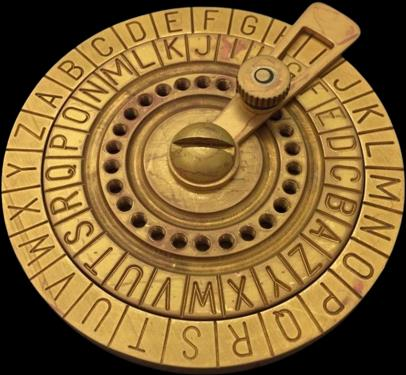
\includegraphics[width=0.85\textwidth]{../../images/python/page_011_img_01.jpeg}

\end{document}
